\chapter{4}


\begin{figure}[h]
\centering
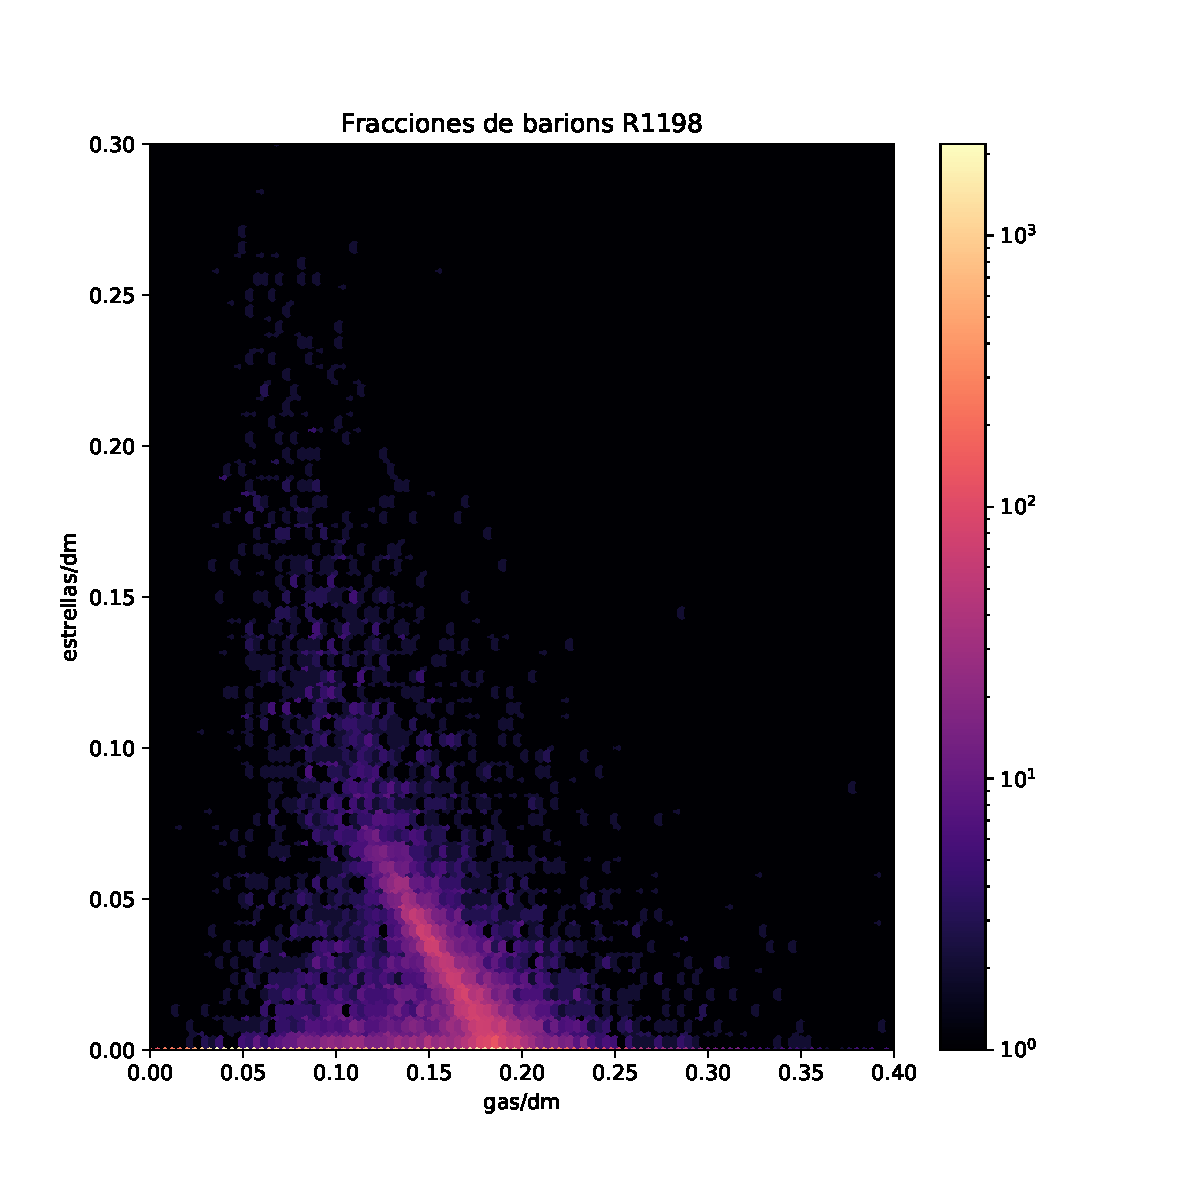
\includegraphics[width=18cm]{Figures/R1198_gas-est_frac.pdf}
\decoRule
\caption[Fraccione stellar vs gas]{Fracciones de gs/dm vs estrellas/dm }
\label{fig:Electron}
\end{figure}

\begin{figure}[h]
\centering
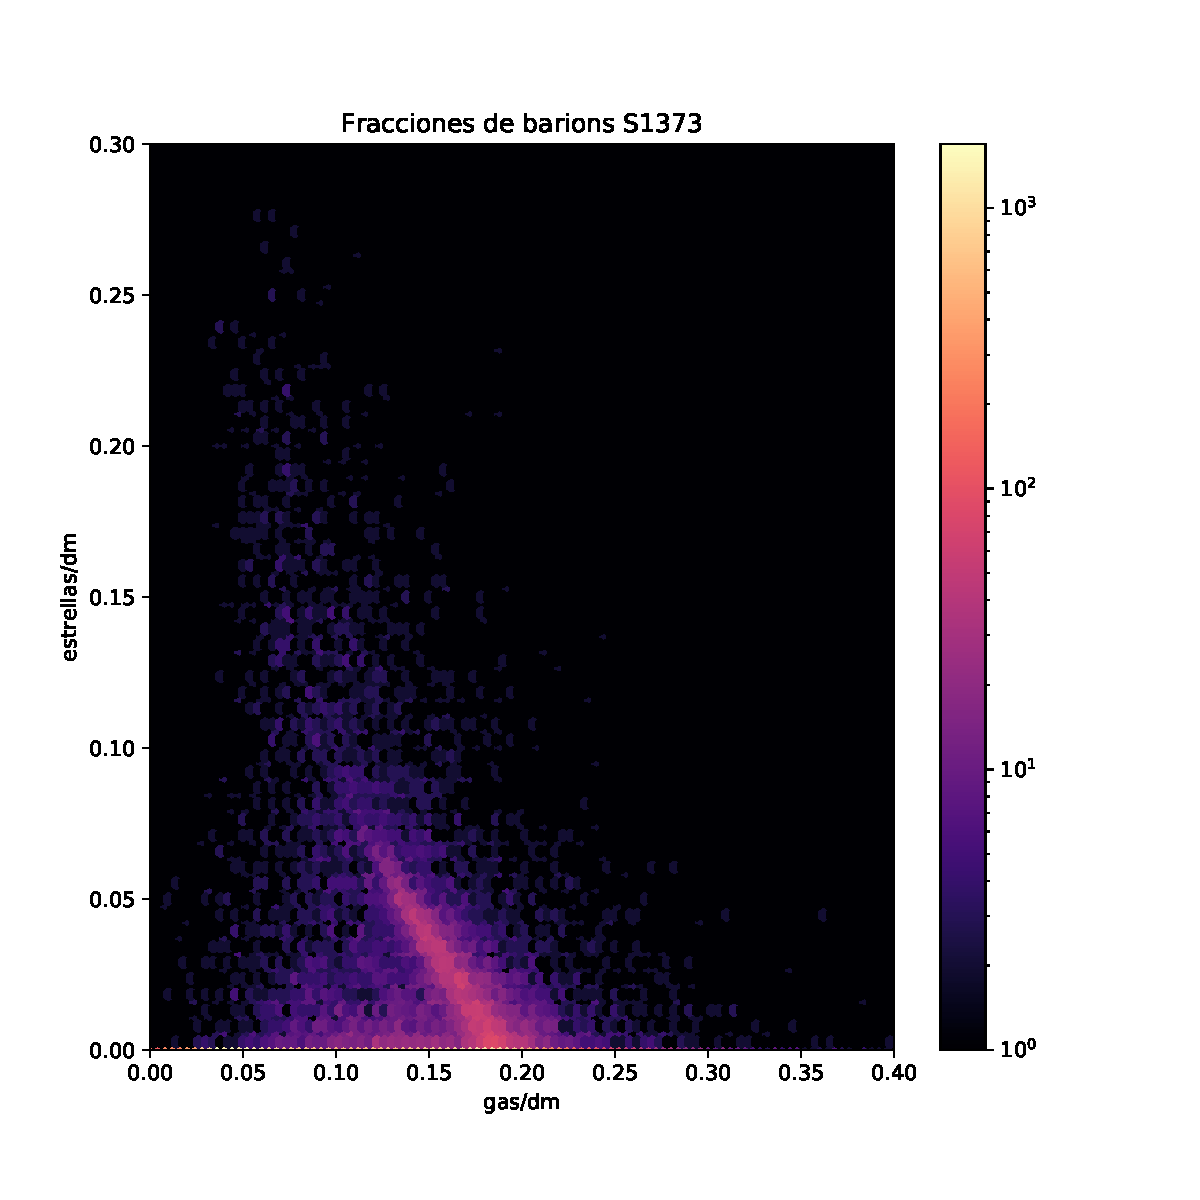
\includegraphics[width=18cm]{Figures/S1373_gas-est_frac.pdf}
\decoRule
\caption[Fraccione stellar vs gas]{Fracciones de gs/dm vs estrellas/dm }
\label{fig:Electron}
\end{figure}

\begin{figure}[h]
\centering
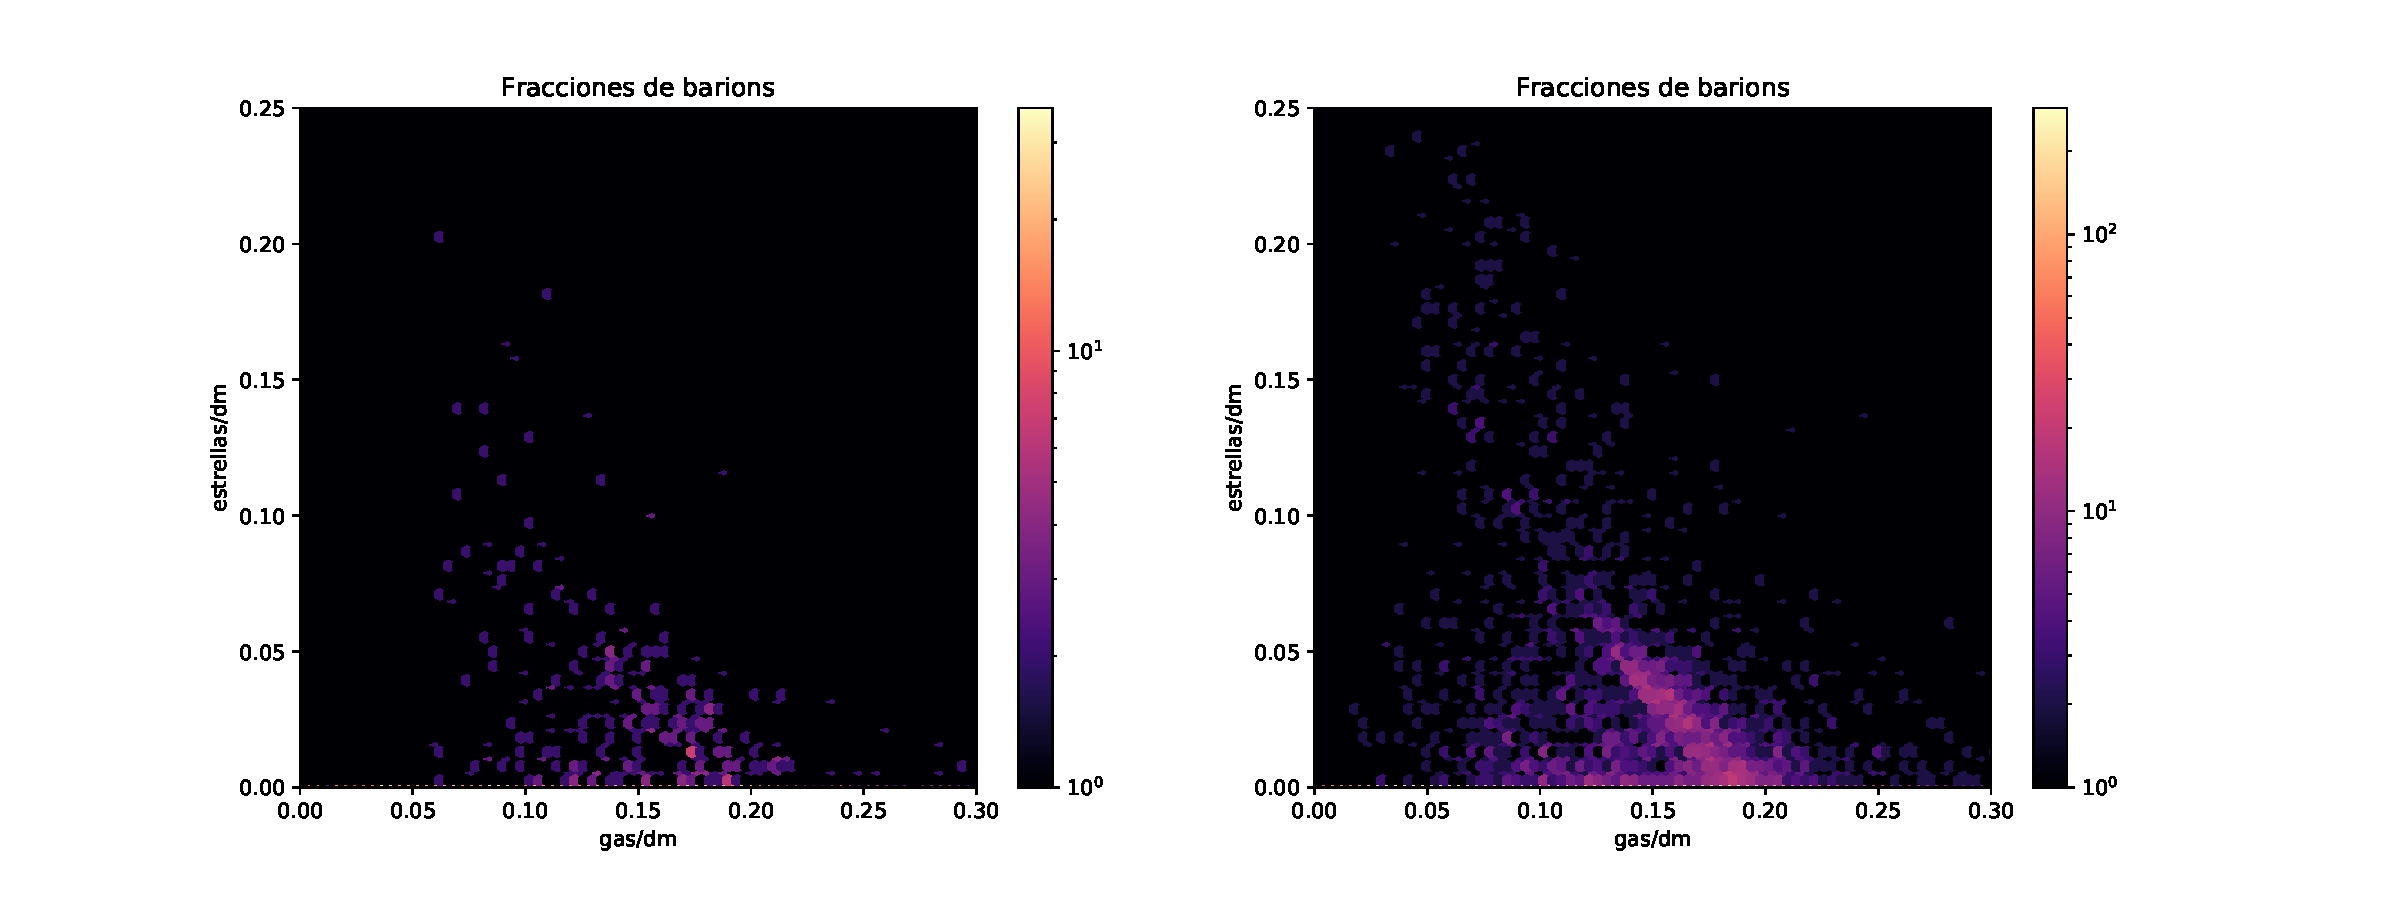
\includegraphics[width=18cm]{Figures/S1373_fraccionesdebarions.pdf}
\decoRule
\caption[Fraccione stellar vs gas]{Fracciones de gs/dm vs estrellas/dm para el VOID (r<10 Mpc y para el entorno r>10}
\label{fig:Electron}
\end{figure}

\begin{figure}[h]
\centering
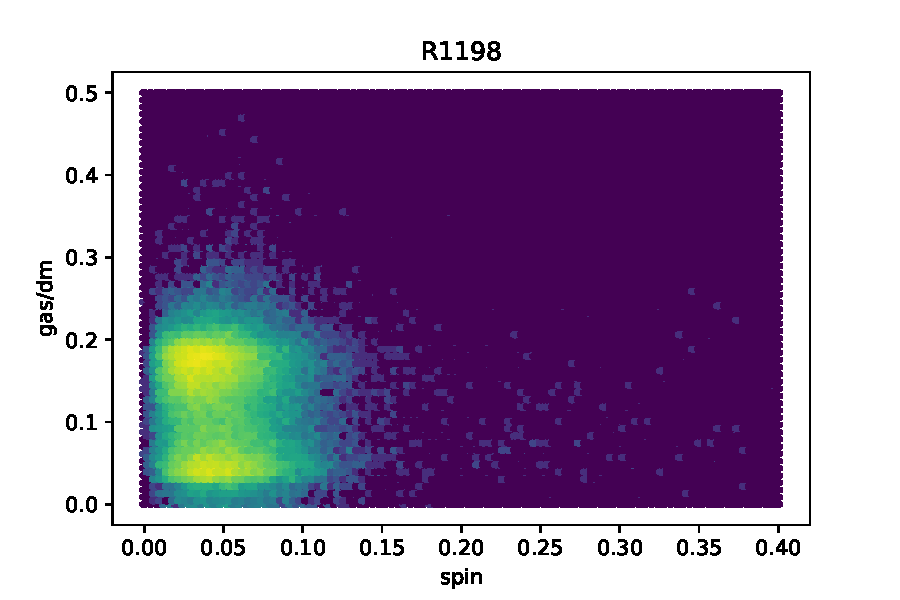
\includegraphics[width=18cm]{Figures/R1198_frac-spin.pdf}
\decoRule
\caption[Fraccione stellar vs gas]{Fracciones de gs/dm vs estrellas/dm para el VOID (r<10 Mpc y para el entorno r>10}
\label{fig:Electron}
\end{figure}

\begin{figure}[h]
\centering
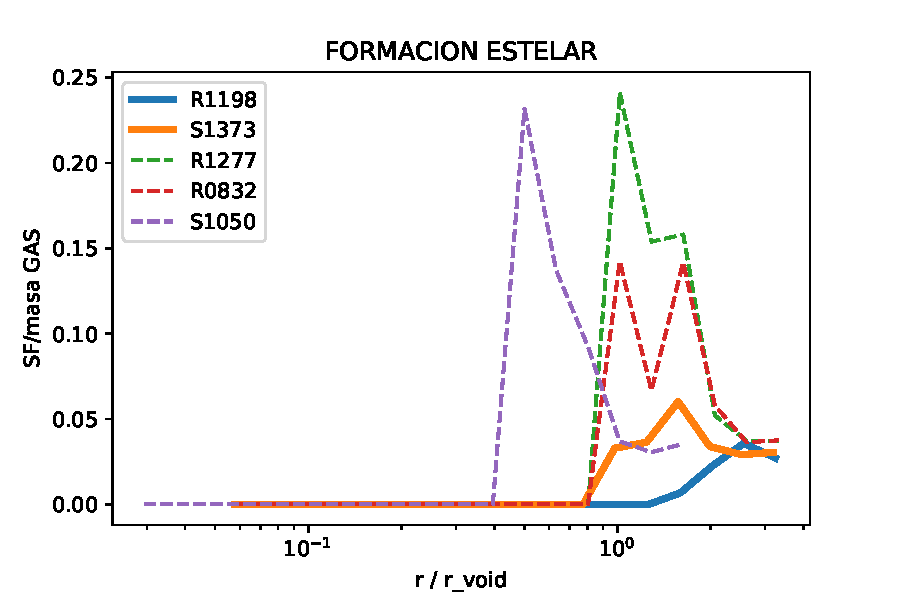
\includegraphics[width=18cm]{Figures/SF.pdf}
\decoRule
\caption[Fraccione stellar vs gas]{Fracciones de gs/dm vs estrellas/dm para el VOID (r<10 Mpc y para el entorno r>10}
\label{fig:Electron}
\end{figure}

\begin{figure}[h]
\centering
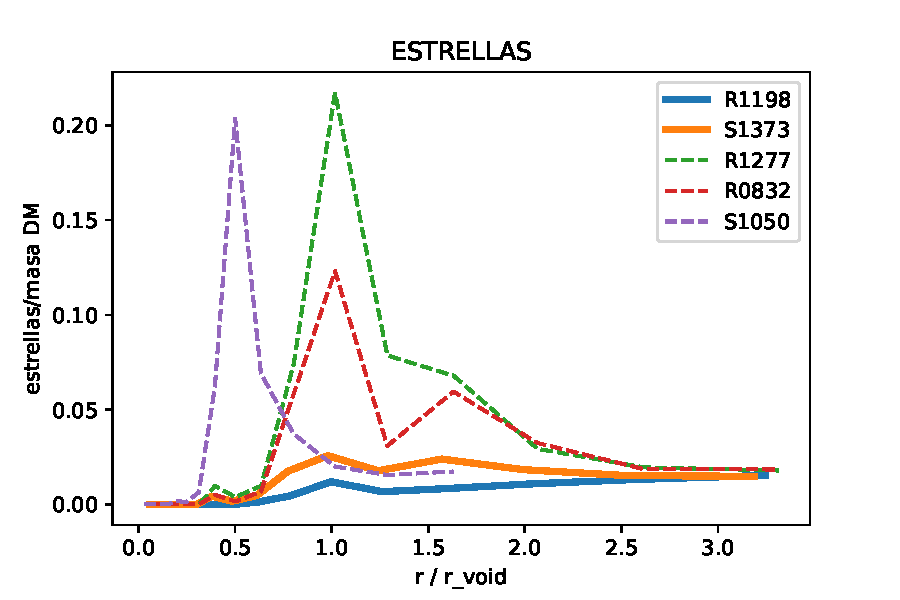
\includegraphics[width=18cm]{Figures/ESTRELLAS.pdf}
\decoRule
\caption[Fraccione stellar vs gas]{Fracciones de gs/dm vs estrellas/dm para el VOID (r<10 Mpc y para el entorno r>10}
\label{fig:Electron}
\end{figure}

\begin{figure}[h]
\centering
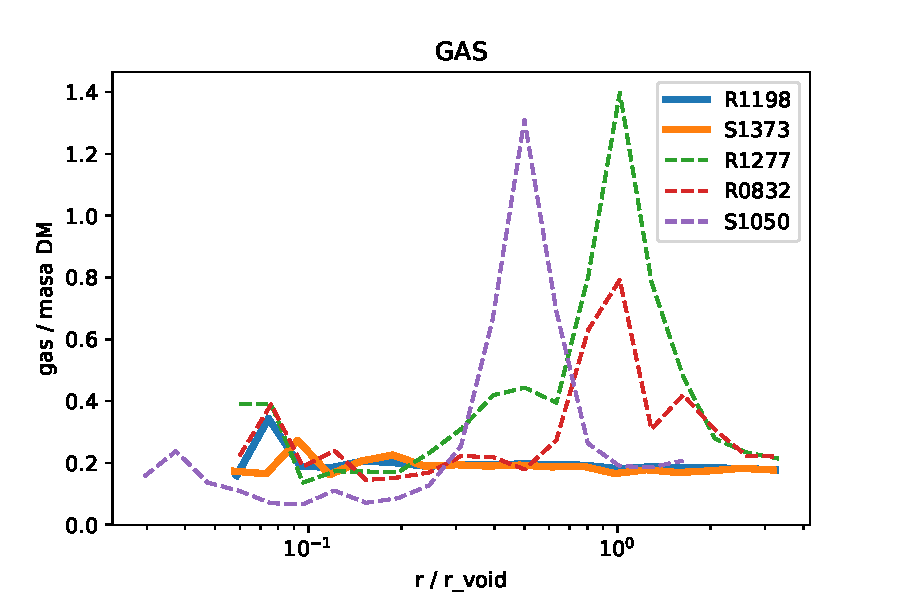
\includegraphics[width=18cm]{Figures/GAS.pdf}
\decoRule
\caption[Fraccione stellar vs gas]{Fracciones de gs/dm vs estrellas/dm para el VOID (r<10 Mpc y para el entorno r>10}
\label{fig:Electron}
\end{figure}

\begin{figure}[h]
\centering
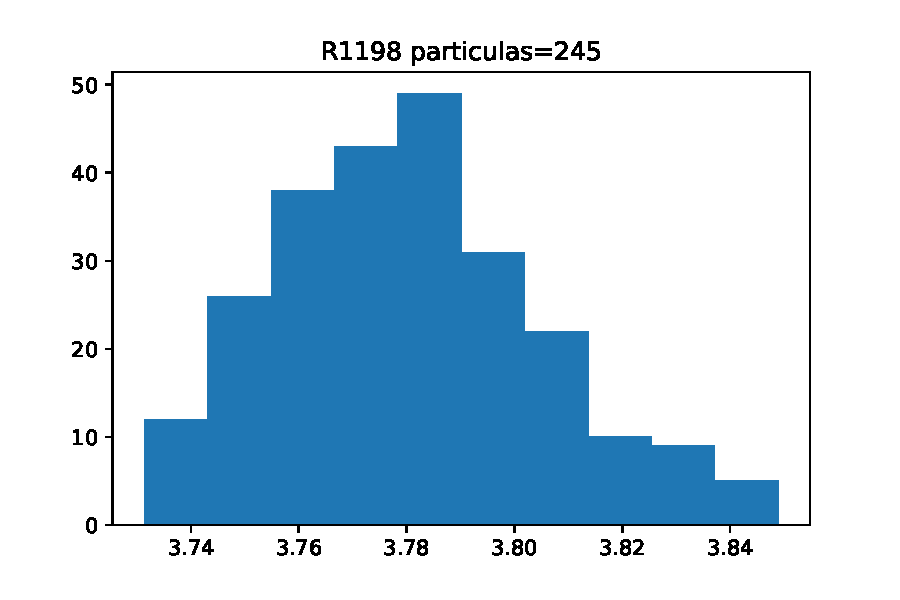
\includegraphics[width=18cm]{Figures/R1198_SFhist.pdf}
\decoRule
\caption[R1198 SF distribucion]{histograma de las 245 particulas de gas con formaci\'on estelar}
\label{fig:Electron}
\end{figure}

\begin{figure}[h]
\centering
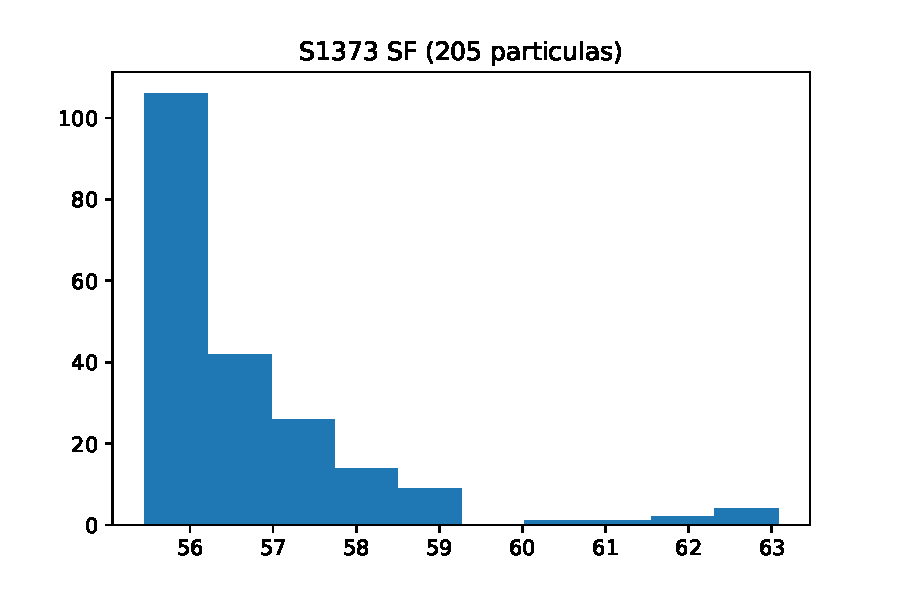
\includegraphics[width=18cm]{Figures/S1373_SFhist.pdf}
\decoRule
\caption[S1373 SF distribucion]{histograma de las 205 particulas de gas con formaci\'on estelar}
\label{fig:Electron}
\end{figure}